\chapter{Extending Classes}

\section{Exercises}

\begin{exercise}
In this exercise, we will explore {\em has-a} and {\em is-a} relationships.

A {\em Has-A} relationship is known as {\em composition}. For example, a \java{Deck} (aggregating class) has a \java{Card} class (aggregated class). So you will expect to see:

\begin{code}
public class Deck {
    private Card[] cards; 
    ...
}
\end{code}

In the UML diagram shown in Figure~\ref{fig.aggregation}, we use an arrow with a diamond head to indicate aggregation, and we can also add notation here that shows that one \java{Deck} contains many \java{Card} objects.

\begin{figure}[!h]
\begin{center}
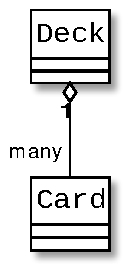
\includegraphics[scale=0.75]{figs/ch14/aggregation.pdf}
\caption{UML Diagram Showing Aggregation - a Deck has Card(s)}
\label{fig.aggregation}
\end{center}
\end{figure}

An {\em Is\-A} relationship is known as {\em inheritance}. For example, a \java{Hand} class (subclass) is also a \java{CardCollection} class (superclass). In Java, we use \java{extends} to indicate inheritance:

\begin{code}
public class Hand extends CardCollection {
   ...
}
\end{code}

Figure~\ref{fig.simpleInheritance} shows the UML for inheritance, using an open arrowhead:

\begin{figure}[!h]
\begin{center}
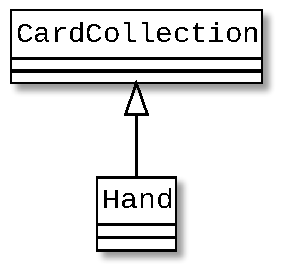
\includegraphics[scale=0.75]{figs/ch14/inheritance.pdf}
\caption{UML Diagram Showing Inheritance - a Hand is a CardCollection}
\label{fig.simpleInheritance}
\end{center}
\end{figure}

First, state whether the relationship of the following classes is composition or inheritance, and draw the UML diagram showing that relationship.

\begin{itemize}
    \item \java{Address} and \java{Student}
    \item \java{Car} and \java{Vehicle}
    \item \java{Account} and \java{SavingsAccount}
    \item \java{State}, \java{Capital}, and \java{Country}
    \item \java{Instructor}, \java{Course}, and \java{Textbook}
    \item \java{Dog}, \java{Cat}, and \java{Animal}
    \item \java{Rectangle}, \java{Circle}, \java{Square}, and \java{Shape}
\end{itemize}


For classes that exhibit the inheritance relationship, could you name a few data fields/attributes for the superclass? Could you name a few for the subclass only?

For example, \java{Teacher} (subclass) is also a \java{Person} (superclass). 
Data fields for \java{Person} are: name, age, address, etc.
Data fields for \java{Teacher} are: school, hire date etc.

\end{exercise}

\begin{exercise}
Design a class named \java{Person} with two subclasses: \java{Employee} and \java{Customer}. The attributes for these classes are described in italics. A \java{Person} has a {\em name}, {\em address}, {\em phone number}, and  {\em email address}.

An \java{Employee} has an {\em employee number}, {\em hire date}, and {\em salary}.

The \java{Employee} class, in turn, has three subclasses: \java{Programmer}, \java{Tester}, and \java{Manager}. 
\begin{itemize}
\item A \java{Programmer} and a \java{Tester} have a {\em cubicle number}. Both will receive a {\em fixed bonus} at the end of the year.
\item A \java{Manager} has an {\em office number} and has a variable bonus based on the performance of their team. This means that a \java{Manager} should have attributes for the {\em target bonus amount} and the {\em performance percentage}.
\end{itemize}

Finally, the \java{Customer} should have a {\em customer number} and {\em company} they work for.

Draw the UML diagram showing the relationship of these classes, then code all these classes showing the data fields and attributes. Make meaningful names for the attributes and give them an appropriate data type. (You do not need to create constructors or other methods for the classes.)
\end{exercise}

\begin{exercise}
The XYZZY Corporation wants to retain their most loyal customers. They launch a customer retention program and offer discount to customers who have been purchasing from the company for at least one year.
<<<<<<< HEAD
Write a subclass \java{PrefCust} that extends the \java{Customer} class from the preceding exercise. The \java{PrefCust} class should have three data fields: {\em purchase amount} and {\em customer history} (number of years they have been a customer), and {\em discount level}. The discount level should depend on the customer history and purchase amount. All of these attributes are private.
=======
>>>>>>> discount

Write a subclass \java{PrefCust} that extends the \java{Customer} class from the preceding exercise. The \java{PrefCust} class should have two data fields: {\em purchase amount} and {\em customer history} (number of years they have been a customer). These are both private variables.

Customers get a discount percentage based on their history and purchase amount. There are three levels of Preferred Customers: bronze, silver and gold.

\begin{itemize}
\item Bronze: history $\geq$ 1 year and average purchase amount $\geq$ \$5000 per year.  5%% off
\item Silver:  history $\geq$ 2 years and average purchase amount $\geq$ \$10000 per year. 7.5%% off
\item Gold:  history $\geq$ 3 years and average purchase amount $\geq$ \$15000 per year. 10%% off
\end{itemize}

The discount percentage is a {\em derived attribute}---it is never set directly, but instead is computed based on other attributes.

Write the \java{PrefCust} class with all its data fields. Please write all the getter and setter methods.  Write a method named \java{getDiscountPercent} that uses the purchase amount and customer history to return the discount percent (as a percentage).
\end{exercise}

%=========================================

\begin{exercise}

In this exercise, you will implement an \java{Account} class which represents a bank checking account. You will then create two classes that inherit from \java{Account}: \java{SavingsAccount} and \java{CreditCardAccount}.

You will then use composition to create a \java{Customer} class which includes instances of each of these account classes.

Finally, you will write a program with a \java{main} method that tests these classes.

{\bf Part 1}: Create a class named \java{Account}, which has the following private properties:

\begin{itemize}
    \item \java{number: long}
    \item \java{balance: double}
\end{itemize}

\begin{enumerate}
\item Create a two-parameter constructor that takes an account number and balance. Make sure that the balance is always greater than zero ({\em Hint}: \java{Math.abs})

\item Implement getters and setters: \java{getNumber()}, \java{getBalance()}, \java{setBalance(double newBalance)}. There is no \java{setNumber} method---once an account is created, its account number cannot change.

\item Implement these methods: \java{void deposit(double amount)} and \java{void withdraw(double amount)}. For both these methods, if the amount is less than zero, the account balance remains untouched. For the \java{withdraw} method, if the amount is greater than the balance, it remains untouched. {\em These methods do not print anything.}

\item Implement a \java{toString} method that returns a string with the account number and balance, properly labeled.
\end{enumerate}

{\bf Part 2}: Next, implement the \java{SavingsAccount} class. It inherits from \java{Account} and adds a private \java{apr} property, which is the annual percentage rate (APR) for interest.

\begin{enumerate}
\item Write a three-argument constructor that takes an account number, balance, and interest rate as a decimal (thus, a 3.5\% interest rate is given as 0.035). Make sure that the interest rate is never less than zero.

\item add a getter and setter: \java{getApr()} and \java{setApr(double apr)}. The setter must ensure that the APR is never less than zero.

\item Write a \java{calculateInterest} instance method that returns the annual interest, calculated as the current balance times the annual interest rate.

\item Modify \java{toString} to include the interest rate. IMPORTANT: The value returned by the \java{toString} method must {\bf {\em not}} include the calculated annual interest.
\end{enumerate}

{\bf Part 3}: Next, implement the \java{CreditCardAccount} class, which inherits from \java{Account} and adds these \java{private} properties:

\begin{itemize}
\item \java{apr}, a \java{double} representing the annual interest rate charged on the balance.
\item \java{creditLimit}, a \java{double} which gives the credit limit for the card.
\end{itemize}

Then, implement:
\begin{enumerate}
\item A four-argument constructor that takes an account number, balance, interest rate as a decimal (thus, a 3.5\% interest rate is given as 0.035), and credit limit. Make sure that neither the interest rate nor credit limit can be negative.

\item Write getters and setters for the \java{apr} and \java{creditLimit}. The apr setter should leave the APR untouched if given a negative value. The \java{creditLimit} setter should leave the credit limit untouched if given a negative value.

\item Modify \java{toString} to include the interest rate and credit limit. IMPORTANT: the value returned by the \java{toString} method must {\bf {\em not}} include the monthly payment.

\item Override the \java{withdraw} method so that you can have a negative balance. If a withdrawal would push you over the credit limit, leave the balance untouched. Examples:

\begin{itemize}
\item If your balance is \$300 with a credit limit of \$700, you can withdraw \$900 (leaving a balance of \$-600).
\item If your balance is \$-300 with a credit limit of \$700, you can withdraw \$350 (leaving a balance of \$-650).
\item If your balance is \$-300 with a credit limit of \$700, you can not withdraw \$500, because that would then owe \$800, which is more than your \$700 limit.
\end{itemize}

In short, the maximum amount you can withdraw is your current balance plus the credit limit.

%\item Implement a \java{calculatePayment} method that works as follows: If the balance is positive, the minimum amount you have to pay on your card per month is zero. Otherwise, your monthly payment is the minimum of 20 and $(apr/12) \cdot (−balance)$

\end{enumerate}

{\bf Part 4}: Now, write a \java{Customer} class that will use composition to include the preceding classes.

\begin{enumerate}
\item The \java{Customer} class has the following private attributes:

\begin{itemize}
\item \java{name: String}
\item \java{acct: Account}
\item \java{savings: SavingsAccount}
\item \java{credit: CreditAccount}
\end{itemize}

\item Implement a four-argument constructor for this class.

\item Write getters and setters for all the fields.
\end{enumerate}

Figure~\ref{fig.inheritance1} shows the details of the \java{Account} class and its subclasses. Figure~\ref{fig.inheritance2} shows the relationships of all the classes in this exercise.

\begin{figure}[!ht]
\begin{center}
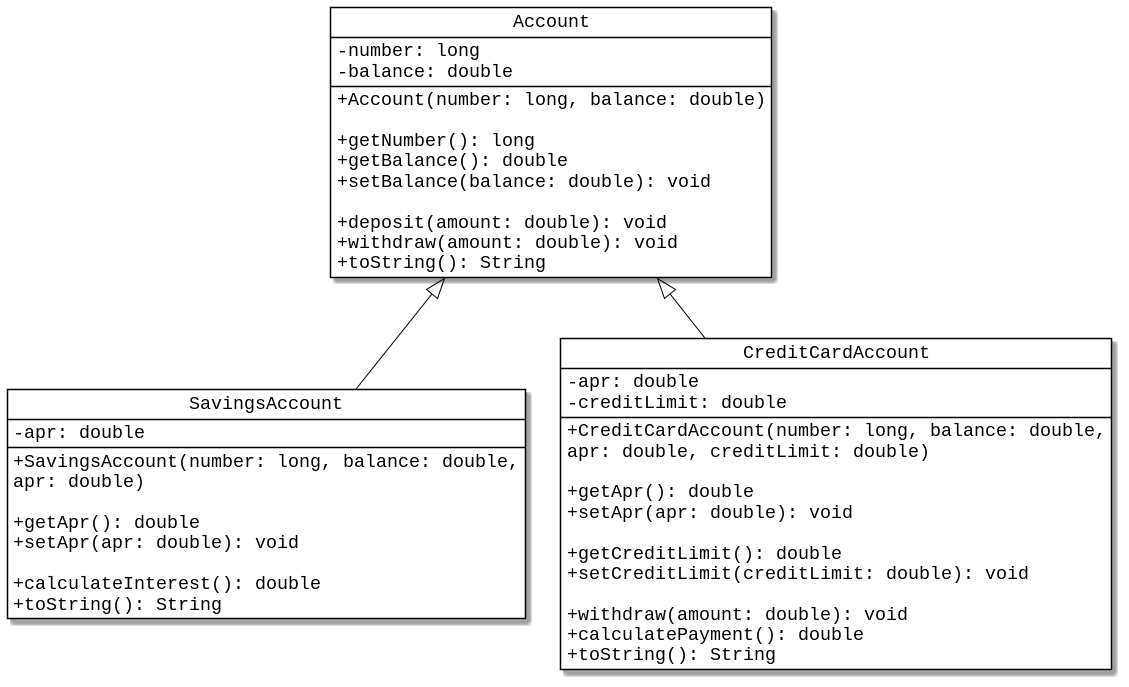
\includegraphics[scale=0.4]{figs/ch14/account_inheritance.png}
\caption{\java{Account}, \java{SavingsAccount}, and \java{CreditCardAccount} classes}
\label{fig.inheritance1}
\end{center}
\end{figure}

\begin{figure}[!ht]
\begin{center}
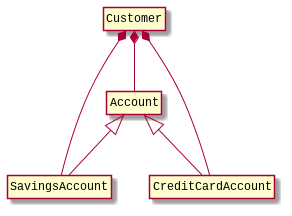
\includegraphics[scale=0.7]{figs/ch14/account_classes.png}
\caption{Composition and Inheritance Among All Classes}
\label{fig.inheritance2}
\end{center}
\end{figure}

{\bf Part 5}: Finally, write a program named {\em TestCustomer.java} that creates a \java{Customer} named ``Joe Doakes'' with this data:

\begin{itemize}
\item Regular account number 1037825 with a balance of \$3,723.00
\item Savings account number 9016632 with a balance of \$4,810.25 and an annual interest rate of 2.05\%
\item Checking account number 85332162 with a balance of -\$2500.00, an interest rate of 7.125\%, and a credit limit of \$3000.00.
\end{itemize}

Then, do the following transactions:

\begin{itemize}
\item Deposit \$257.18 into the regular account, then withdraw \$587.23.
\item Deposit \$2,466.12 into the savings account, then withdraw \$8,000.00.
\item Withdraw \$480.00 from the credit card account.
\item Display the status of the regular account (number and balance).
\item Display the status of the savings account (number, balance, and annual interest amount).
\item Display the status of the credit card account (number, balance, interest rate, and monthly payment due).
\end{itemize}


\end{exercise}
